%\documentclass[wcp,gray]{jmlr} % test grayscale version
\documentclass[wcp]{jmlr}% former name JMLR W\&CP
%\documentclass[pmlr]{jmlr}% new name PMLR (Proceedings of Machine Learning)

 % The following packages will be automatically loaded:
 % amsmath, amssymb, natbib, graphicx, url, algorithm2e
 \usepackage{amsmath,amssymb,graphicx,url}

 %\usepackage{rotating}% for sideways figures and tables
\usepackage{longtable}% for long tables

 % The booktabs package is used by this sample document
 % (it provides \toprule, \midrule and \bottomrule).
 % Remove the next line if you don't require it.
\usepackage{booktabs}
 % The siunitx package is used by this sample document
 % to align numbers in a column by their decimal point.
 % Remove the next line if you don't require it.
\usepackage[load-configurations=version-1]{siunitx} % newer version
 %\usepackage{siunitx}

% Package to make table with multi rows and columns
\usepackage{multirow}
 
 % to do
\usepackage{xcolor}
\newcommand\todo[1]{\textcolor{red}{#1}}

 % change the arguments, as appropriate, in the following:
\jmlrvolume{}
\jmlryear{}
\jmlrworkshop{STA723 -- Case Study 1}
\jmlrproceedings{}{}


\usepackage[toc,page]{appendix}


% start article
% \titlebreak
% \footnote{}
% \textsf

\title[DDE and PCB effect on Premature delivery]{Assessing Effects of Exposures to DDE and PCBs on Premature Delivery via Ordinal Logistic Regression}	%\titletag{\thanks{XXX}} % leave empty?

 % Use \Name{Author Name} to specify the name.
 % If the surname contains spaces, enclose the surname
 % in braces, e.g. \Name{John {Smith Jones}} similarly
 % if the name has a "von" part, e.g \Name{Jane {de Winter}}.
 % If the first letter in the forenames is a diacritic
 % enclose the diacritic in braces, e.g. \Name{{\'E}louise Smith}

 % Authors with different addresses:
 
 \author[Morsomme, Ou, Zito]{Raphael Morsomme \and Rihui Ou \and Alessandro Zito}
 \date{\today} % Date, can be changed to a custom date

 % Three or more authors with the same address:
 % \author{\Name{Author Name1} \Email{an1@sample.com}\\
 %  \Name{Author Name2} \Email{an2@sample.com}\\
 %  \Name{Author Name3} \Email{an3@sample.com}\\
 %  \addr Address}

 % Authors with different addresses:
 % \author{\Name{Author Name1} \Email{abc@sample.com}\\
 % \addr Address 1
 % \AND
 % \Name{Author Name2} \Email{xyz@sample.com}\\
 % \addr Address 2
 %}

% leave editor's section empty?
%\editor{Editor's name}
% \editors{List of editors' names}

\begin{document}

\maketitle

\textcolor{red}{NEED AN ABSTRACT HERE}
%\begin{abstract} \end{abstract}
\newpage
%%%%%%%%%%%%%%%%%%%%%%%%%%%%%%%%%%%%%%%%%%%%%%%%%%%%%%%%%%%%%
% INTRODUCTION
%%%%%%%%%%%%%%%%%%%%%%%%%%%%%%%%%%%%%%%%%%%%%%%%%%%%%%%%%%%%%
\section{Introduction}
\label{sec:intro}

Dichlorodiphenyldichloroethylene (DDE) and Polychlorinated Biphenyls (PCB) are two chemical elements which were commonly useD in the United States for agricultural purpouses and were banned during the 70's due to their detrimental effect on human health. In particular, exposure to these chemical products has been linked to neurobehavioral and developmental deficits in newborns. As the human body stores them in its fatty tissues, studying their impact on human health is particularly important.

In this report, we examine the effect of DDE and PCB on fetuses; more precisely, we assess the potential association between the exposure to these chemicals and the chance of early delivery. Ideally, a higher exposure to the substances induces a preterm delivery, which may have adverse consequences for the child. To verify this theory, we construct an ordinal logistic regression model over three delivery groups defined by the recorded lenght of the gestation period.  We find that the impact of the substances is essentially race specific: exposure to DDE increases the risk of early childbirth among white people and exposure to PCB increases the risk among non-white ones. 

The report is divided as follows: \sectionref{sec:method} presents the data and our methodology,  \sectionref{sec:results} reports our findings, \sectionref{sec:conclusion} discusses the results and concludes.


%%%%%%%%%%%%%%%%%%%%%%%%%%%%%%%%%%%%%%%%%%%%%%%%%%%%%%%%%%%%%
% METHODS
%%%%%%%%%%%%%%%%%%%%%%%%%%%%%%%%%%%%%%%%%%%%%%%%%%%%%%%%%%%%%
\section{Methods}
\label{sec:method}

\subsection{Data}
\label{sec:data}
The data set consists of 2,380 pregnant women that visited a hospital during their pregnancy in 2001. It contains the length of the gestation in weeks, the concentration doses of DDE and the twelve PCB breakdown products in the blood, the concentration of cholesterol and triglycerides and several demographic information (race, level of education, income, occupation, age, smoking status and the center attended by the woman). However, 43 women showed a length of gestation superior to 45 weeks (the second longest gestation period ever recorded), and 1 women did not show any records of the PCBs levels. Thus, we decide to drop them, reducing the number of women to 2,336. Finally, we mean impute the missing data on the income, education and occupational scores\footnote{Note that these scores will not end up in the final model.}. The following subsection describes the construction of the relevant variable in our analysis.

\subsection{Feature Engineering}
As a first step, we divide the women into three groups, labelled as "Dangerous Preterm", "Preterm" and "At term" based upon the lenght of thei gestation (shorter than $33$ weeks, between $34$ and $36$ weeks and longer than $37$ weeks, respectively). The groups are mean to capture the danger associated to the birth for the child himself. While a delivery after 37 weeks is considered normal, the main organs (especially the respiratory system) develop between week 34 and 37, making a birth before 34 weeks more dangerous. Second, as the twelve PCB measurements showed a high correlation (see \figureref{fig:corr}), we aggregate them into a unique variable by taking their standardized average \footnote{We first standardize each single PCB to to prevent one measurement to dominate the aggregate variable.}. Third, we combine the measurements of chemical in blood with the fat-related variables to estimate the initial level of DDE and PCBs to which the women were exposed from the environment. In particular, we calculate the total amount of fatty tissues using the formula in \textcolor{red}{PHILLIPS (1989) BERNET (2007)}

\begin{equation}
\label{eq:fat}
\text{lipid} = 2.27 * \text{cholesterol} + \text{triglycerides} + 0.623.
\end{equation}
Then, since the amount of chemical absorbed is proportional to the amount of fatty tissue one has, we divide the concentration of PCB and DDE in blood by the log of the level of lipid\footnote{This correction derives from a Box-Cox analysis of our model, following the basic procedure in (\textcolor{red}{LI LONGNECKER DUNSON (2013)}). See the appendix for further details.}.
\begin{equation}
\label{eq:exp_dde_pcb}
\text{DDE}_{\text{exposure}} = \dfrac{\text{DDE}}{\log(\text{lipid})} \qquad \text{PCB}_{\text{exposure}} = \dfrac{\text{PCB}_\text{aggregate}}{\log(\text{lipid})}.
\end{equation}
Finally, we aggregate the women into two groups, "white" and "non-white", based on the reported race\footnote{The original data had 1,016 white women, 1,201 black ones, and 120 labelled as "other". As the categories a unbalanced, we prefer to merge for a clearer interpretation.}.

\subsection{Model}
$\text{DDE}_{\text{exposure}}$ and $\text{PCB}_{\text{exposure}}$ are our variables of interest, whereas the above contructed delivery group is our dependent variable. In order to identify non-spurious association between these variables and the occurrence of early deliveries, we run the following ordinal logistic regression model 

\begin{equation}
\label{eq:ordi_logit}
\end{equation}
\todo{
Since not all attributes are necessarily related to the dependent variable, we conduct an backward AIC-based variable selection procedure. Ideally, we would have preferred to avoid selecting variables and instead run a BMA, but since Merlise's package does not allow ordinal logistic regression, we opted for the simpler frequentist approach. The variable selection procedure includes XXXX and drops XXXXX. We use the variables selected y the procedure as predictors in a Bayesian ordinal logistic regression model. The model was fit using stan. We use $10$ chains of $10,000$ iterations each, and put a uniform prior on the coefficients.}

%%%%%%%%%%%%%%%%%%%%%%%%%%%%%%%%%%%%%%%%%%%%%%%%%%%%%%%%%%%%%
% RESULTS
%%%%%%%%%%%%%%%%%%%%%%%%%%%%%%%%%%%%%%%%%%%%%%%%%%%%%%%%%%%%%
\section{Results}
\label{sec:results}

%%%%%%%%%%%%%%%%%%%%%%%%%%%%%%%%% EDA
\subsection{EDA}
\textcolor{red}{RAPHAEL: MAKE 3 SENTENCES IN WHICH YOU SUMMARIZE THE PLOTS IN THE EDA.}



%%%%%%%%%%%%%%%%%%%%%%%%%%%%%%%%% MAIN FINDINGS
\subsection{Main Findings}
\textcolor{red}{RIHUI: MAKING A LISTED DOT LIKE WE DID IN THE SLIDES IS NOT A GOOD IDEA WHEN YOU HAVE TO SUMMARIZE EVERYTHING IN THREE PAGES. THIS SECTION NEEDS TO BE REVISED.}
Main findings: the effect of the chemicals on the risk of early delivery is race dependent. Exposure to DDE has a particularly detrimental impact on the gestation process among white women, while exposure to PCB affects non-white more (see \figureref{fig:results})).
We gave the 90\% credible intervals for coefficients and their posterior mean. (Table \ref{tab:confints}). The interpretation of coefficients are as follow:
\begin{itemize}
	\item $\text{DDE}_{\text{exposure}}$: For a 1 unit increase of $\text{DDE}_{\text{exposure}}$, holding other covariates constant,
		    \begin{itemize}
		    	\item \textbf{Nonwhite}: the odds of having a more dangerous delivery increase by $(e^{(0.02)}-1)*100\%=2.02\%$. The 90\% credible interval is $[-2.00\%, 4.12\%]$.
		    	\item \textbf{White}:  the same odds increase by $(e^{(0.02+0.05)}-1)*100\%=7.25\%$
		    \end{itemize}
	\item $\text{PCB}_{\text{exposure}}$: For a $0.1$ unit increase of $\text{PCB}_{\text{exposure}}$, holding other covariates constant,
			\begin{itemize}
				\item \textbf{Nonwhite}: the odds of having a more dangerous delivery increase by $(e^{(1.76)*0.1}-1)*100\%=19.22\%$. The 90\% credible interval is $[6.47\%,30.65\%]$.
				\item \textbf{White}:  the same odds increase by $(e^{0.1*(1.76-1.60)}-1)*100\%=1.595\%$
			\end{itemize}
\end{itemize}

%%%%%%%%%%%%%%%%%%%%%%%%%%%%%%%%% SENSITIVITY ANALYSIS
\subsection{Sensitivity Analysis}
\textcolor{red}{RIHUI: WE NEED TO RUN THE BAYESIAN MODEL WITH A DIFFERENT PRIOR. AND COMMENT ON THE RESULTS HERE. \\
RAPAHEL: SHOULD WE INCLUDE THE FREQUENTIST ESTIMATES ASWELL?}
\section{Conclusions and further discussion}
\label{sec:conclusion}

Future, add quadratic term to age since gestations at a young and an old age are more at risk of complications.

Consider interaction between PCB and DDE

\newpage
%%%%%%%%%%%%%%%%%%%%%%%%%%%%%%%%% PLOTS OF EDA
\section*{Exploratory Data Analysis}
\textcolor{red}{RAPHAEL: ADD GRAPHS FOR THE EDA. IDEALLY, WE NEED THE TWO GRAPHS IN THE SLIDES, AND THE CORRELATION AMONG THE PCBs. TRY TO FIT THEM IN ONE PAGE.}
\begin{figure}[htbp]
	\floatconts
	{fig:corr}
	{\caption{Correlation among the 12 PCBs variables.}}
	{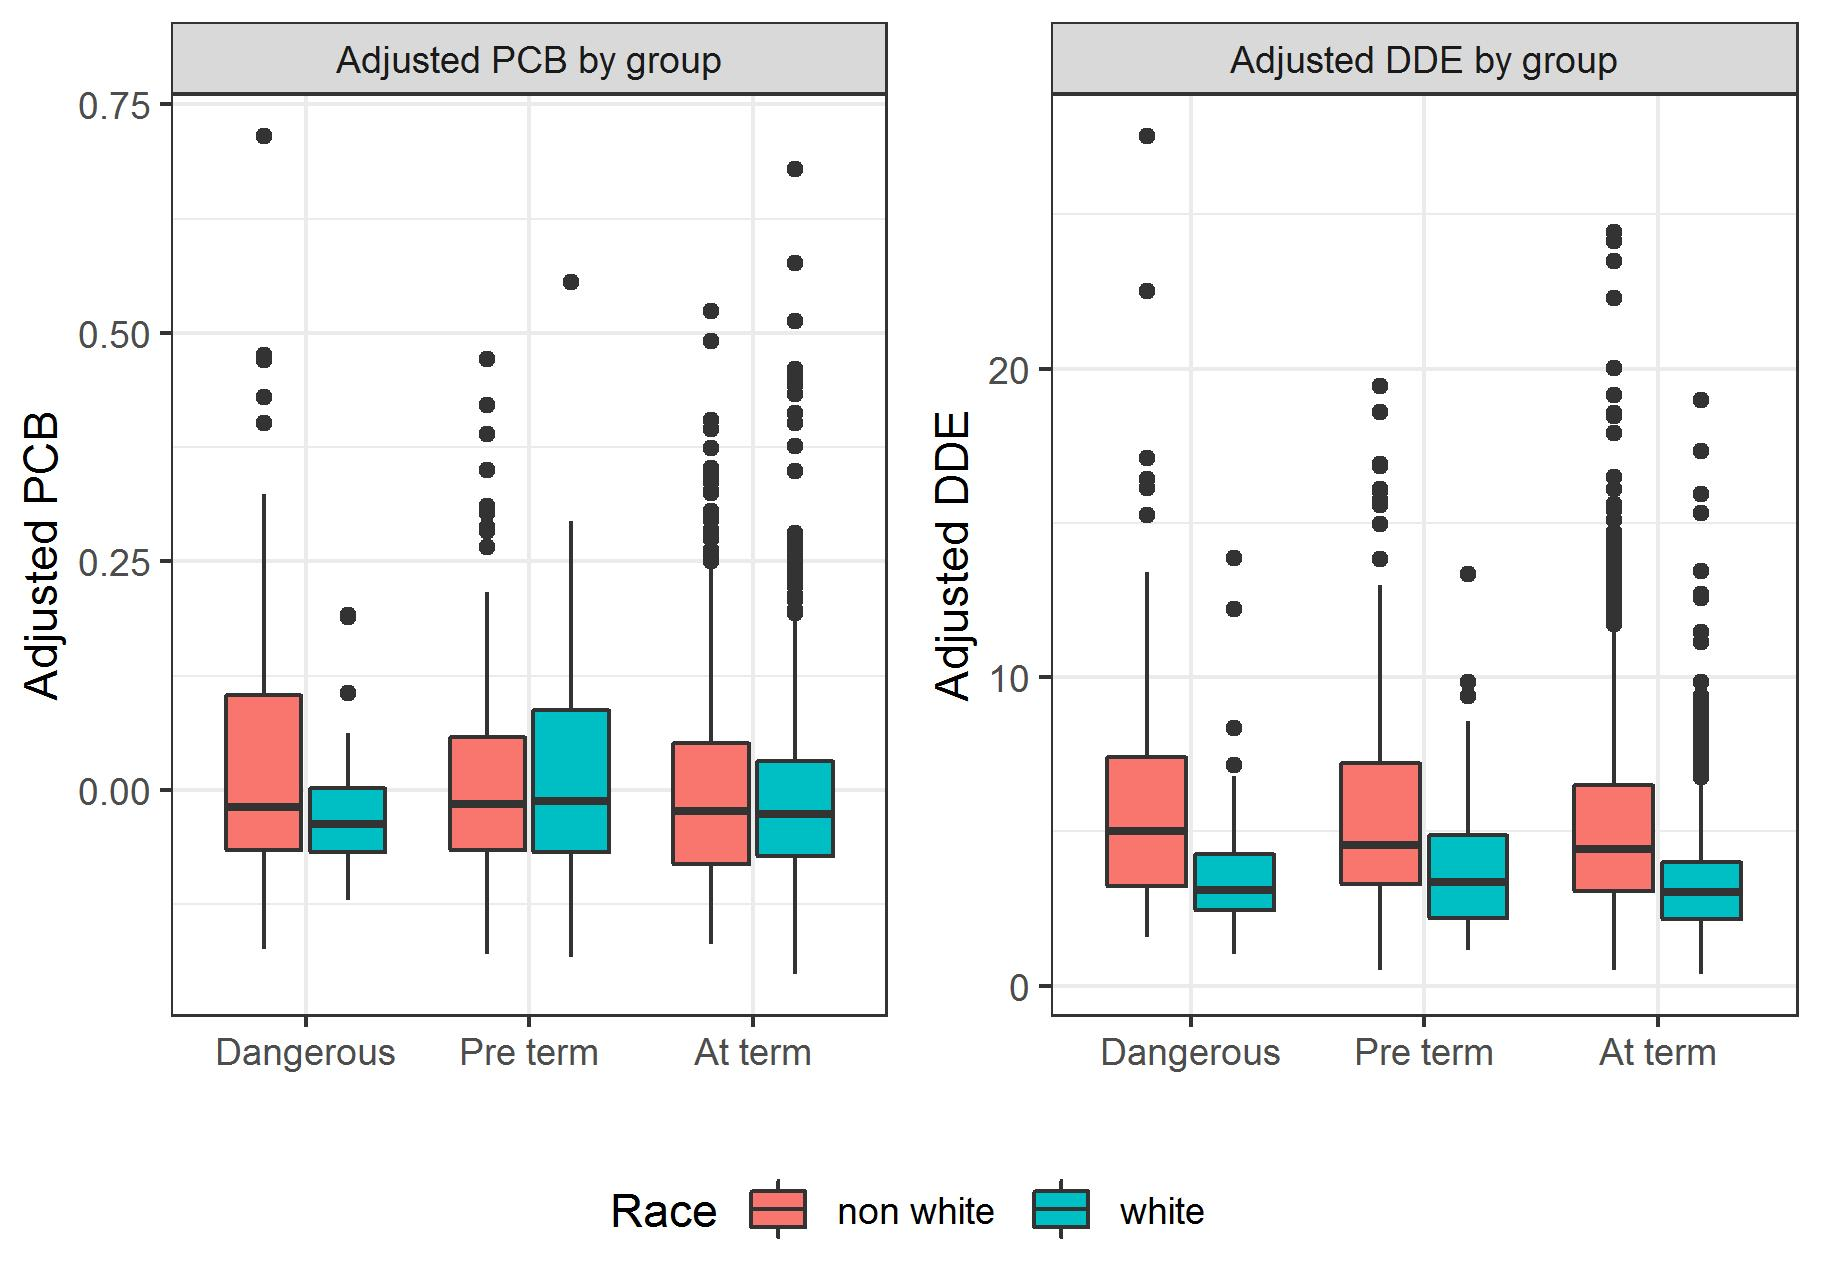
\includegraphics[width=0.8\linewidth]{pcb_corr}}
\end{figure}

%%%%%%%%%%%%%%%%%%%%%%%%%%%%%%%%% TABLES AND PLOTS OF MODEL RESULTS
\section*{Model Results}
\begin{table}
	\centering
	\begin{tabular}{l|r|r|r}
		\hline
		& mean & 5\% & 95\%\\
		\hline
		$\text{DDE}_{\text{exposure}}$ & 0.02 & -0.01 & 0.05\\
		\hline
		$\text{PCB}_{\text{exposure}}$& 1.76 & 0.72 & 2.75\\
		\hline
		$\text{DDE}_{\text{exposure}}$*white & 0.05 & -0.02 & 0.12\\
		\hline
		$\text{PCB}_{\text{exposure}}$*white & -1.60 & -3.26 & 0.02\\
		\hline
	\end{tabular}
    \caption{\label{tab:confints} 90\% credible intervals and posterior mean of coefficients}
\end{table}
\textcolor{red}{RAPHAEL: THIS TABLE NEEDS TO BE MADE PRETTIER. SHOULD WE REPORT MORE COEFFICIENTS?}

\begin{figure}[htbp]
	\floatconts
	{fig:corr}
	{\caption{Estimated probability of gestation outcomes in function of race, and exposure to DDE and PCB.}}
	{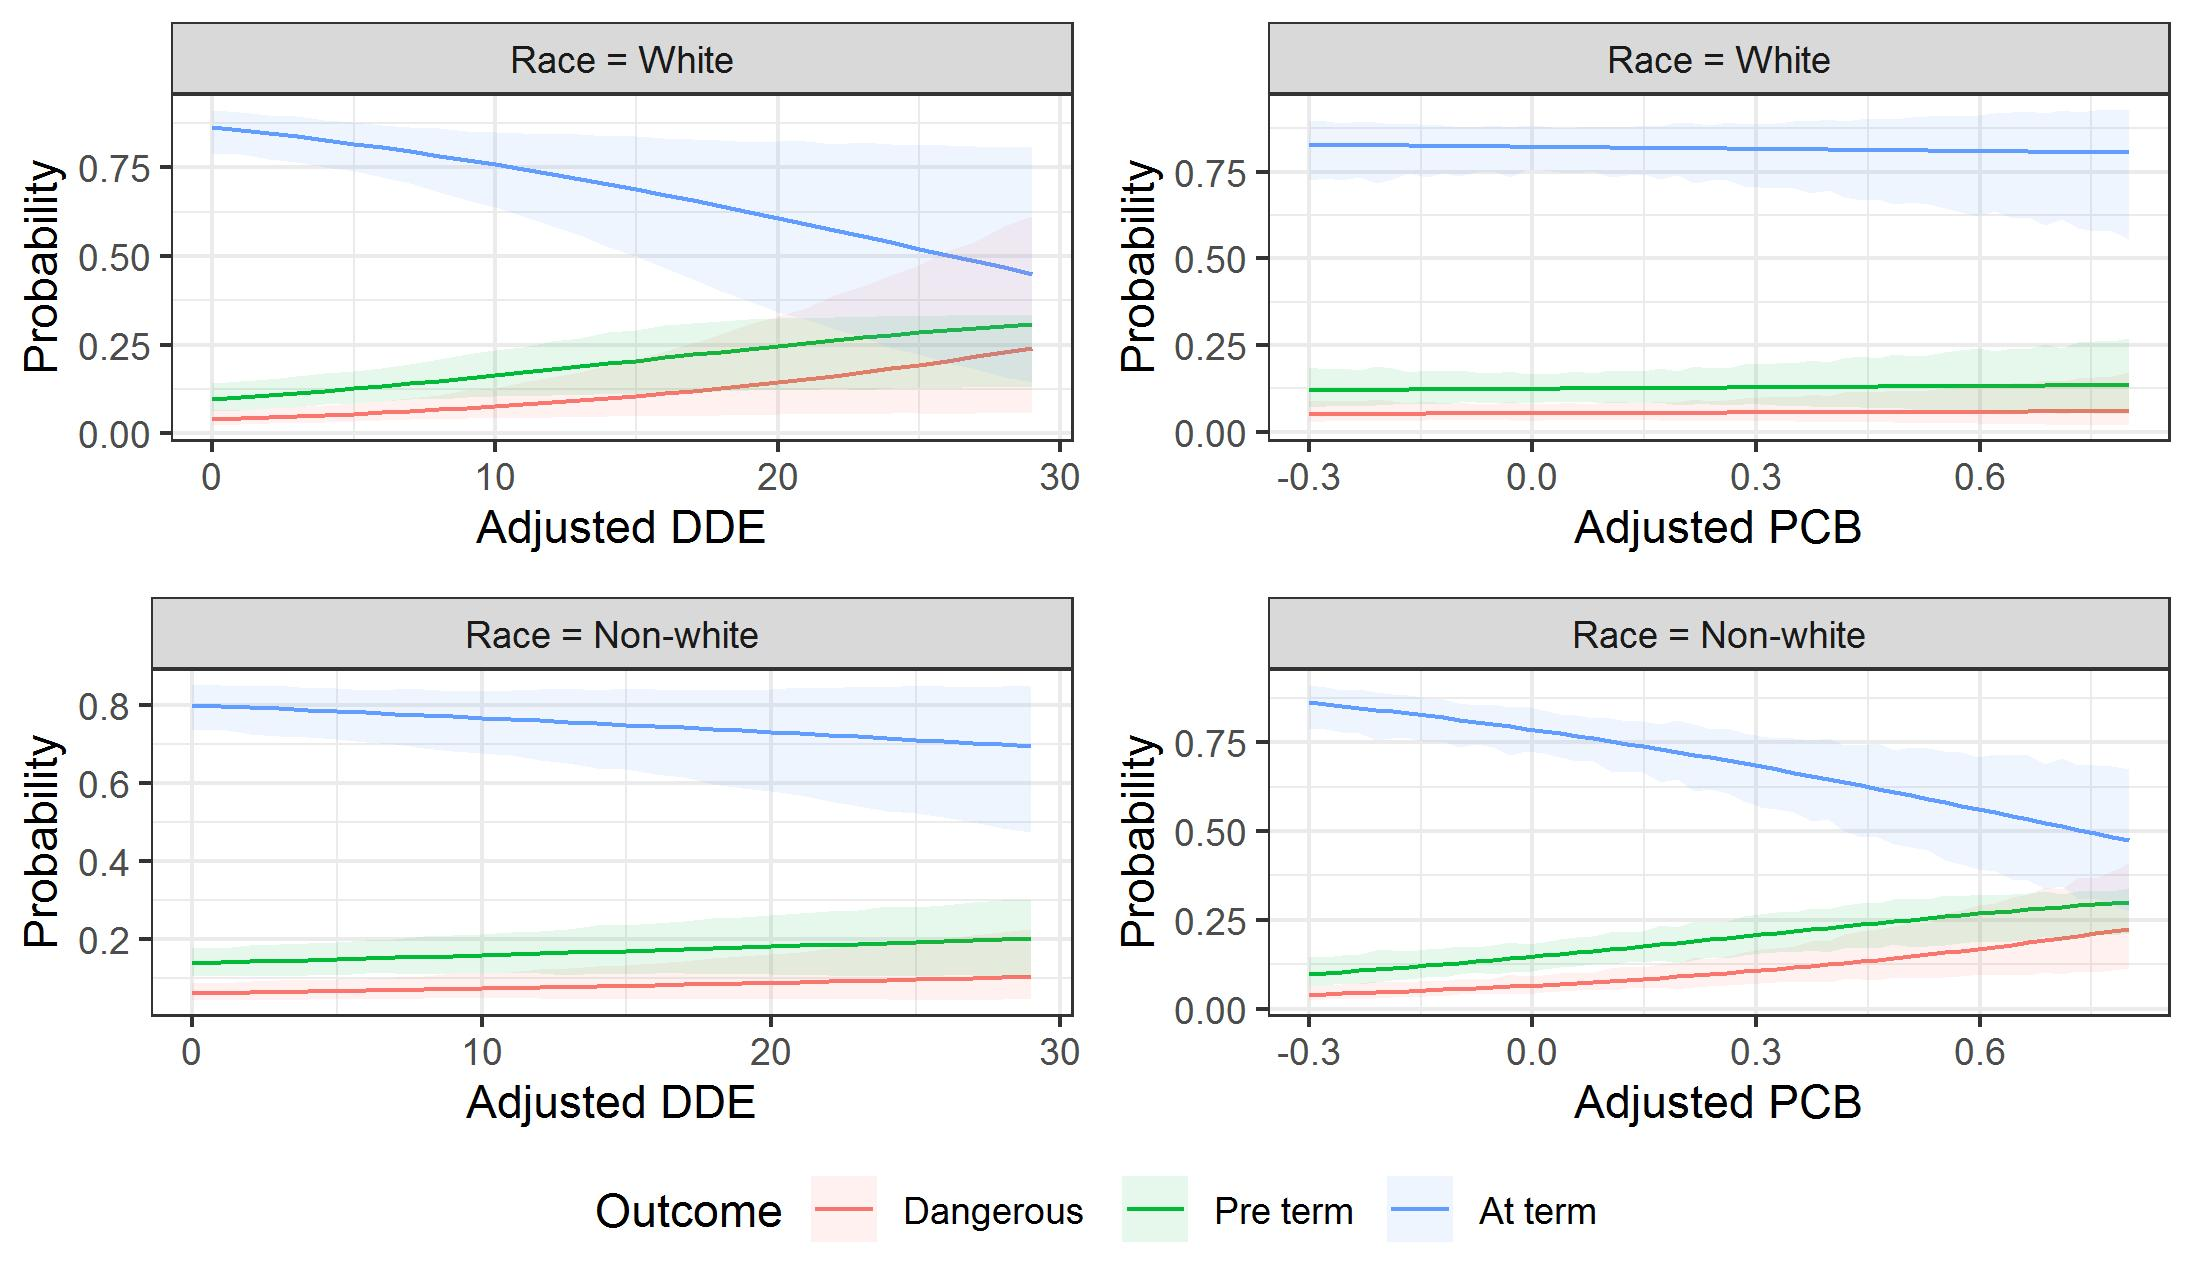
\includegraphics[width=0.8\linewidth]{results}}
\end{figure}

\textcolor{red}{ADD HERE THE SAME PLOT UNDER A R2 PRIOR.}

%%%%%%%%%%%%%%%%%%%%%%%%%%%%%%%%%%%%%%%%%%%%%%%%%%%%%%%%%%%%%
% APPENDIX
%%%%%%%%%%%%%%%%%%%%%%%%%%%%%%%%%%%%%%%%%%%%%%%%%%%%%%%%%%%%%
\newpage
\appendix
\section{Appendix}
%%%%%%%%%%%%%%%%%%%%%%%%%%%%%%%%% BOX COX
\subsection{Box-Cox analysis for lipid adjustment.}
\textcolor{red}{ALESSANDRO'S JOB}
%%%%%%%%%%%%%%%%%%%%%%%%%%%%%%%%% AIC VARIABLE SELECTION
\subsection{Variable selection procedure}
\textcolor{red}{RIHUI'S JOB. WE NEED TO SHOW THE RESULT OF OUR AIC CODE. MORE IN GENERAL, WE NEED TO SHOW SOME FREQUENTIST RESULTS.}
%%%%%%%%%%%%%%%%%%%%%%%%%%%%%%%%% MODEL CHECKING
\subsection{Model Checking}
\textcolor{red}{RIHUI'S JOB. FIX IT AND MAKE IT BETTER READABLE. WHAT ARE THE SURROGATE RESIDUALS? WE NEED AN EXPLANATION. THIS IS NOT SUFFICIENT.}

Since the ordinal data is used here, the common residual plot model checking is not applicable here. Instead, the surrogate residual method suggested by (%$\ref{zz2017}$
) is used. If the model assumption is satisfied, the surrogate residual $R_S$ should display three features: 

\begin{enumerate}
	\item $E(R_S|X)=0$
	\item $Var(R_S|X)=c$, the conditional variance of $R_S$ is constant
	\item The emprical distribution of $R_S$ resembles an explicit distribution that is related to the link function $G^{-1}(\cdot)$. Specifically, $R_S\sim G(c+\int ud G(u))$.
\end{enumerate}

The scatterplot (Figure\ref{fig:surrogateresid}) indicates that feature 1 and 2 are roughly satisfied. The QQ plot indicates that feature 3 is roughly satisfied, although the tail of our sample distribution is lighter than that of the theoretical one. 

\begin{figure}
	\centering
	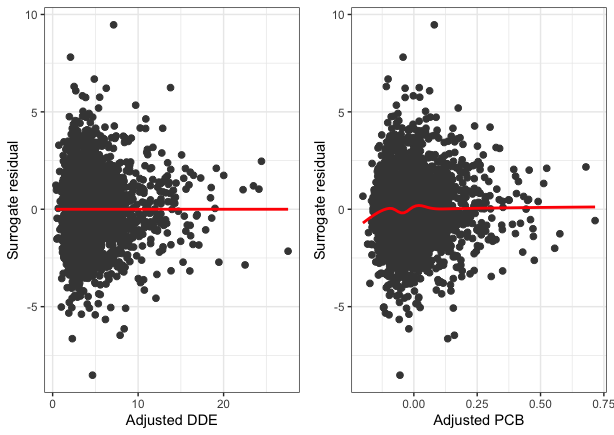
\includegraphics[width=0.7\textwidth]{Surrogate_residuals.png}
	\caption{Surrogate residuals of DDE and PCB}
	\label{fig:surrogateresid}
\end{figure}

\begin{figure}
	\centering
	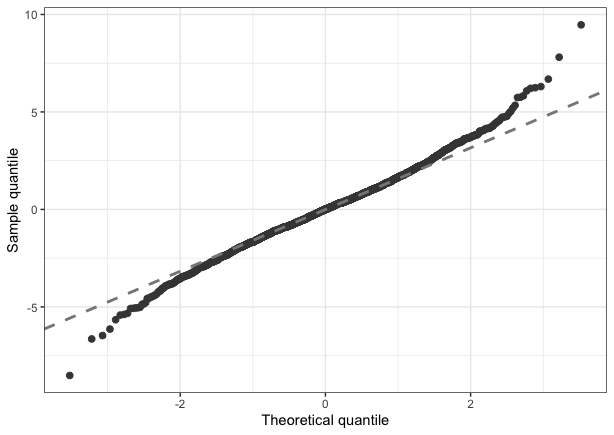
\includegraphics[width=0.7\textwidth]{qqplot.png}
	\caption{QQ plot of the Surrogate residuals}
	\label{fig:qqplot}
\end{figure}



%\bibliography{bibliography}
\end{document}